\begin{figure}[ht]
    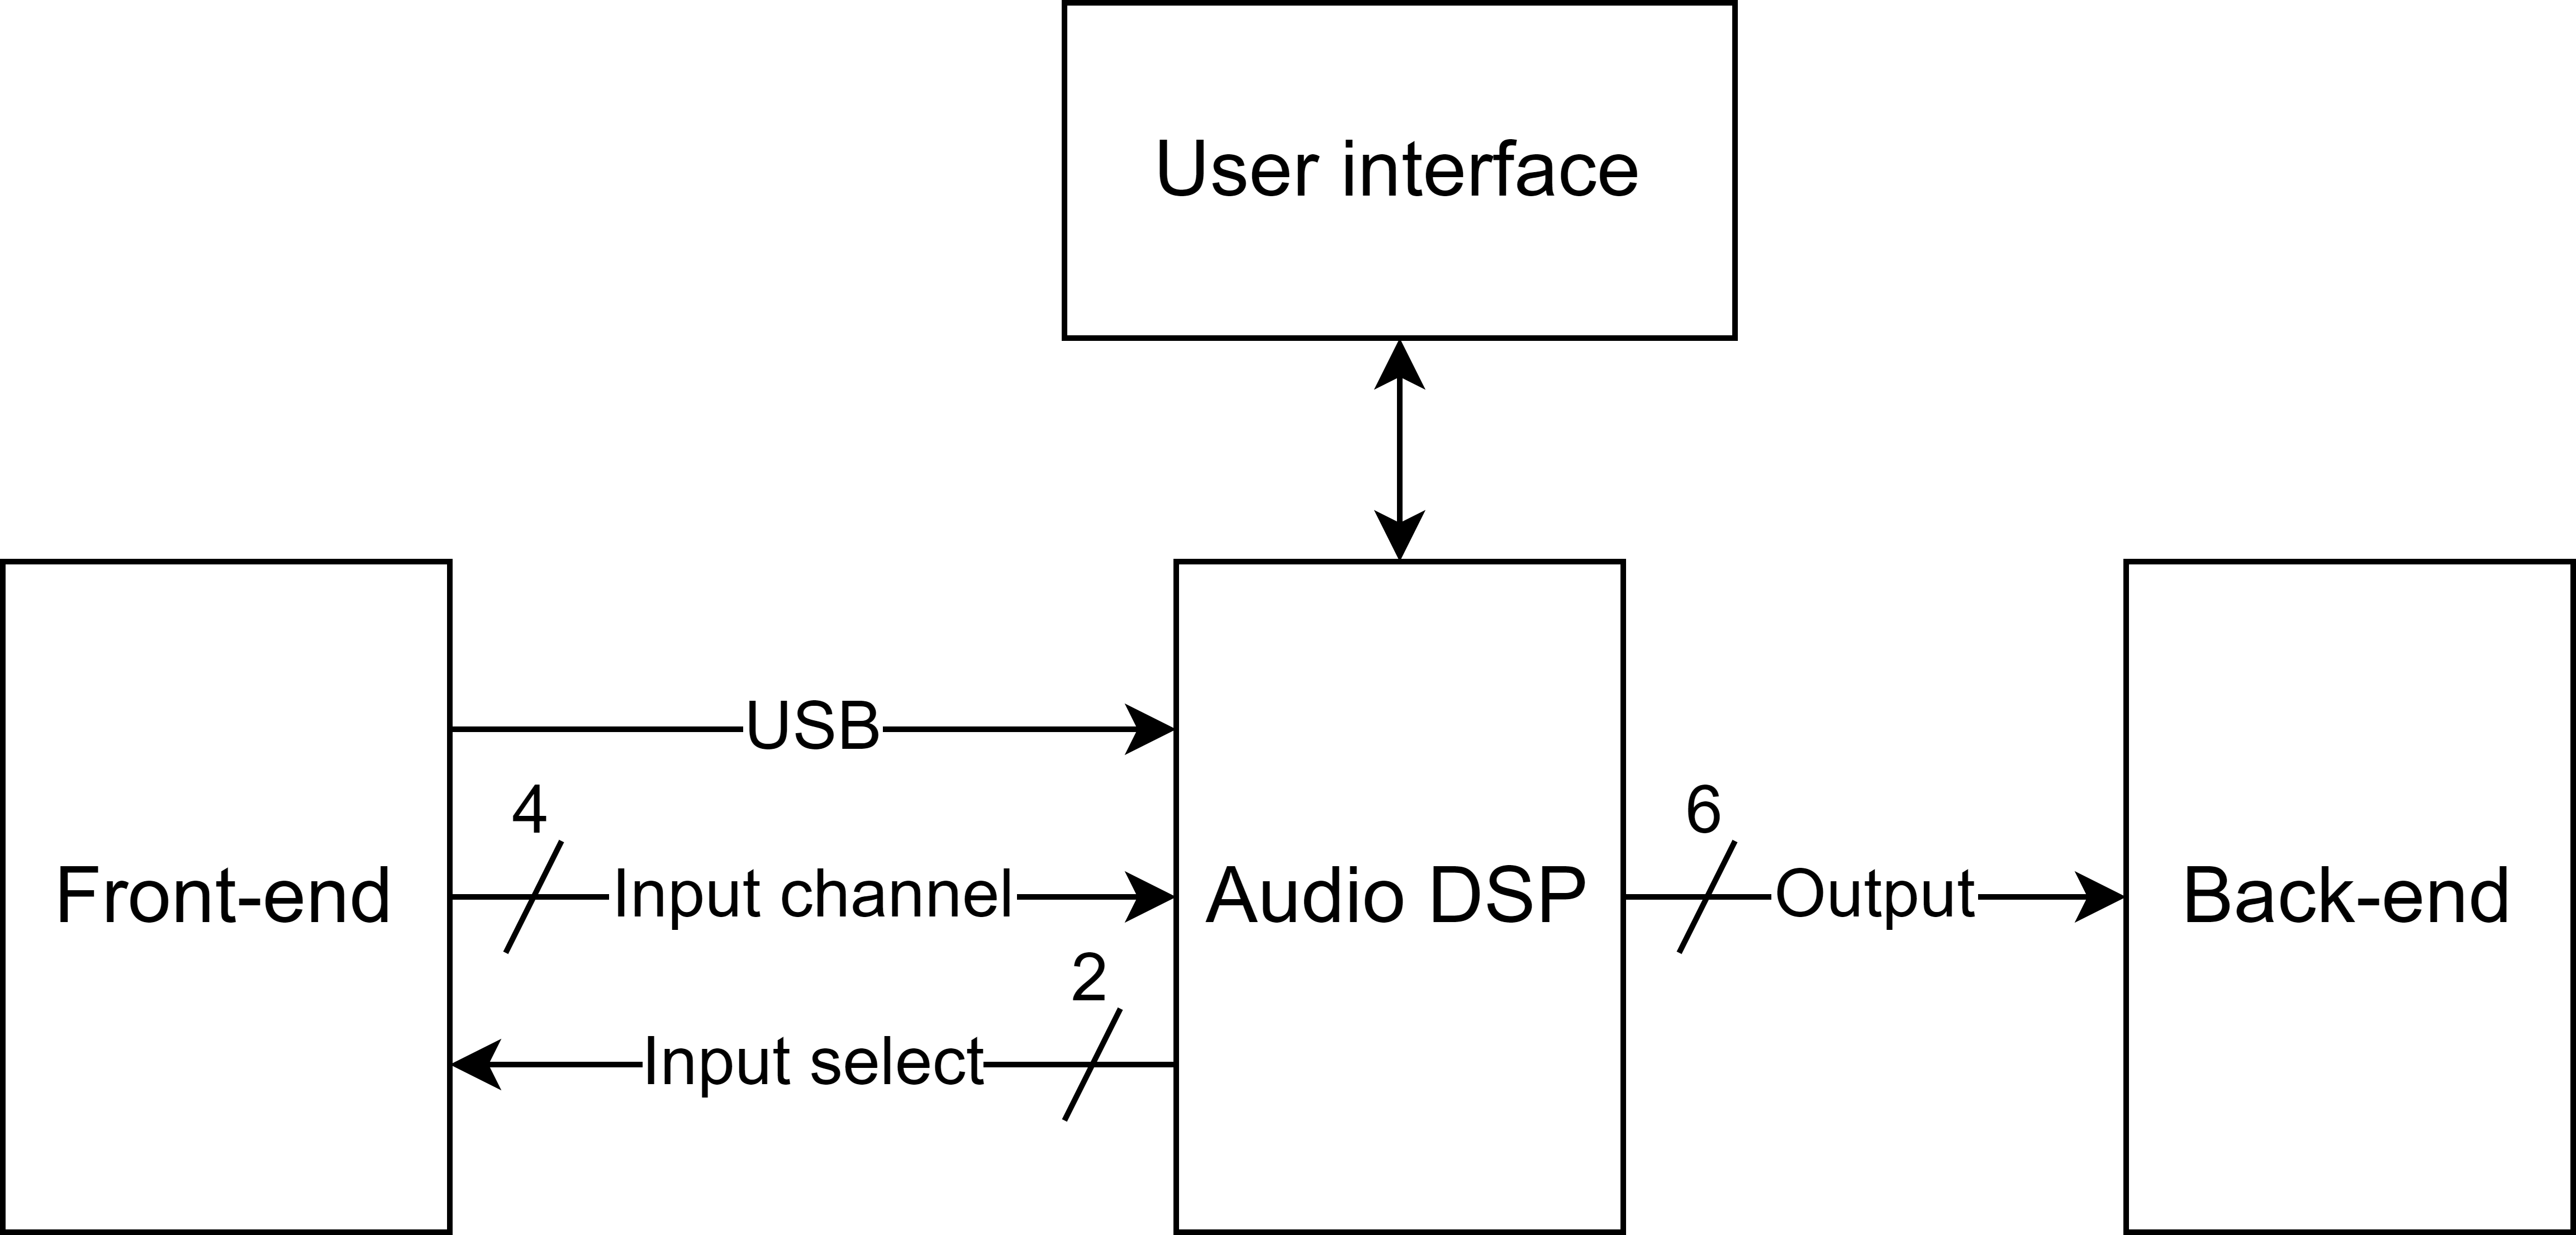
\includegraphics[width=\linewidth]{System context-top level.png}
    \caption{System context diagram of the top-level}
    \label{fig:sys-context-top}
\end{figure}

After the system requirement document has been approved, the system context diagram could be made (see figure \ref{fig:sys-context-top}). The block called "Audio DSP" is the heart of the system. This block represents the controller and thus the FPGA core. This system context design diagram fulfills all the requirements, including the should and could haves. Therefore the Audio-DSP has four analogue inputs, one USB input and six analogue outputs. The input select line is for selecting what line input you want on input channel 1 and 2. The user can either select a RCA or 6.35mm jack input on input channel 1 and 2.

With a user interface the user is able to configure the effect parameters, equalizer settings and volume of each channel. The user is also able to rearrange the position of effects in the effects loop per channel.

\section{Front-end}
\begin{figure}[ht]
    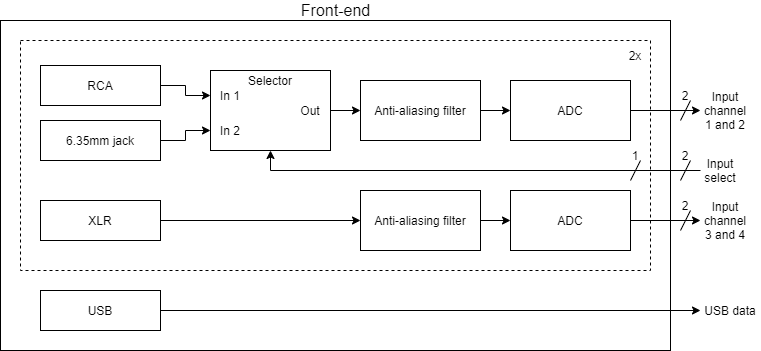
\includegraphics[width=\linewidth]{System context-front-end.png}
    \caption{System context diagram of front-end design}
    \label{fig:system-context-front-end}
\end{figure}

The front end block Is a physical representation of how the front end of the system will function (see figure \ref{fig:system-context-front-end}). The user will be able to use four different type of connectors to connect to the audio-DSP, these connections are: RCA, XLR, 6.35mm jack and USB. The user will be able to select on the user interface witch connector will be used. The analogue signal will than be filtered and modified to meet the specifications of the input of the ADC. Than the ADC will convert the signal to the digital domain where it can be used for signal processing. 

\section{Audio-DSP}
\begin{figure}[ht]
    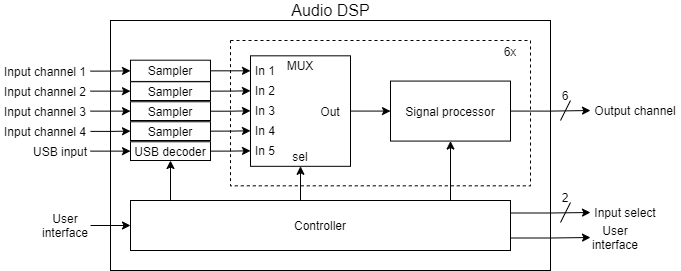
\includegraphics[width=\linewidth]{System context-audio DSP.png}
    \caption{System context diagram of Audio-DSP}
    \label{fig:sys-context-audio-dsp}
\end{figure}

The Audio-DSP block is made in the digital domain of the system (see figure \ref{fig:sys-context-audio-dsp}). Therefore this block will be made in the FPGA. Each analogue input signal needs to be sampled in order for the system to be able to process the data. Thus each analogue input signal has a sampler block. The USB input signal has an USB decoder block as a sampler. 

After the sampler blocks each sampled signal goes to six channels with each a 5 to 1 MUX (multiplexer). With this MUX the user is able to select what input signal will be processed in each channel. The chosen signal will then go to the signal processor block. In the signal processor block the input signal will be modified by the various configurable effects, equalizer and volume settings. These effects, equalizer and volume configurations can be configured by the user via the user interface.

After the signal has been modified by the signal processor block it will be fed out of the FPGA to the back-end of the system.

\section{Back-end}
\begin{figure}[ht]
    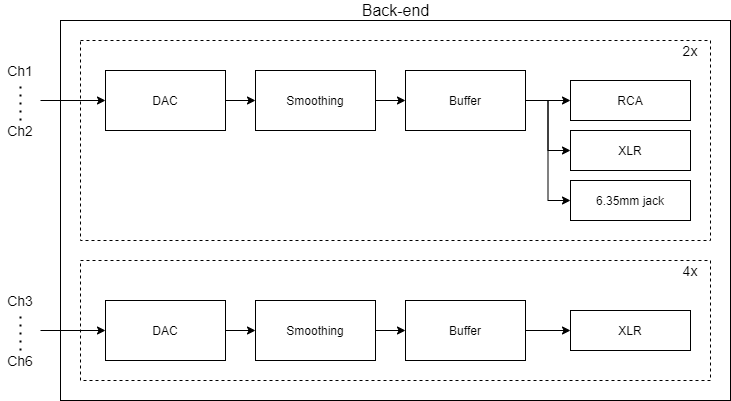
\includegraphics[width=\linewidth]{System context-back-end.png}
    \caption{System context diagram of back-end}
    \label{fig:system-context-back-end}
\end{figure}

The back end block is a physical representation of how the back end of the system will function (see figure \ref{fig:system-context-back-end}). The user will be able to use three outputs for the signal. These connections are: RCA, XLR and 6.35mm jack. The user will be able to select the right output in the user interface. There will be six output channels. Four are only XLR and two will have to option to be either XLR, RCA or 6.35mm jack. After the FPGA has processed the signal it will be converted back to analogue using a DAC, then the signal will be filtered and buffered to meet the specifications of the selected connectors.

\section{Interfacing}
As described in the System Requirements Document (SRD), the audio DSP must include multiple input and output connectors and a user friendly user interface (UI).
\subsection{Inputs}
The system includes the following inputs:
\begin{itemize}
    \item DC jack to power the system
    \item CH1 RCA or jack
    \item CH2 RCA or jack
    \item CH3 XLR
    \item CH4 XLR
    \item CH5 USB (optional)
\end{itemize}

\subsection{Outputs}
Output channels 1 and 2 provide the most flexibility as each channel features a balanced XLR output as well as a parallel-connected RCA and jack input. Therefore, the RCA and jack input always carry precisely the same signal. Output channels 3 through 6 exclusively have balanced XLR outputs. The audio DSP, therefore, has the following outputs:

\begin{itemize}
    \item CH1 XLR, RCA and jack
    \item CH2 XLR, RCA and jack
    \item CH3 XLR
    \item CH4 XLR
    \item CH5 XLR
    \item CH6 XLR
\end{itemize}

\subsection{User interface}
Through the UI, the following settings can be configured by the user:
\begin{itemize}
    \item Input selection between RCA or jack for CH1 and CH2.
    \item Channel routing, determining which input is used by each output.
    \item The number and types of filters used can be adjusted.
    \item The filter coefficients can be set.
\end{itemize}

\subsection{Overview}
A black box representation of the audio-DSP is shown in figure \ref{fig:Black-box-rep}. The diagram illustrates the audio DSP's connections to the outside world, providing the highest-level overview of the system through the black box diagram.
\begin{figure}[ht]
    \centering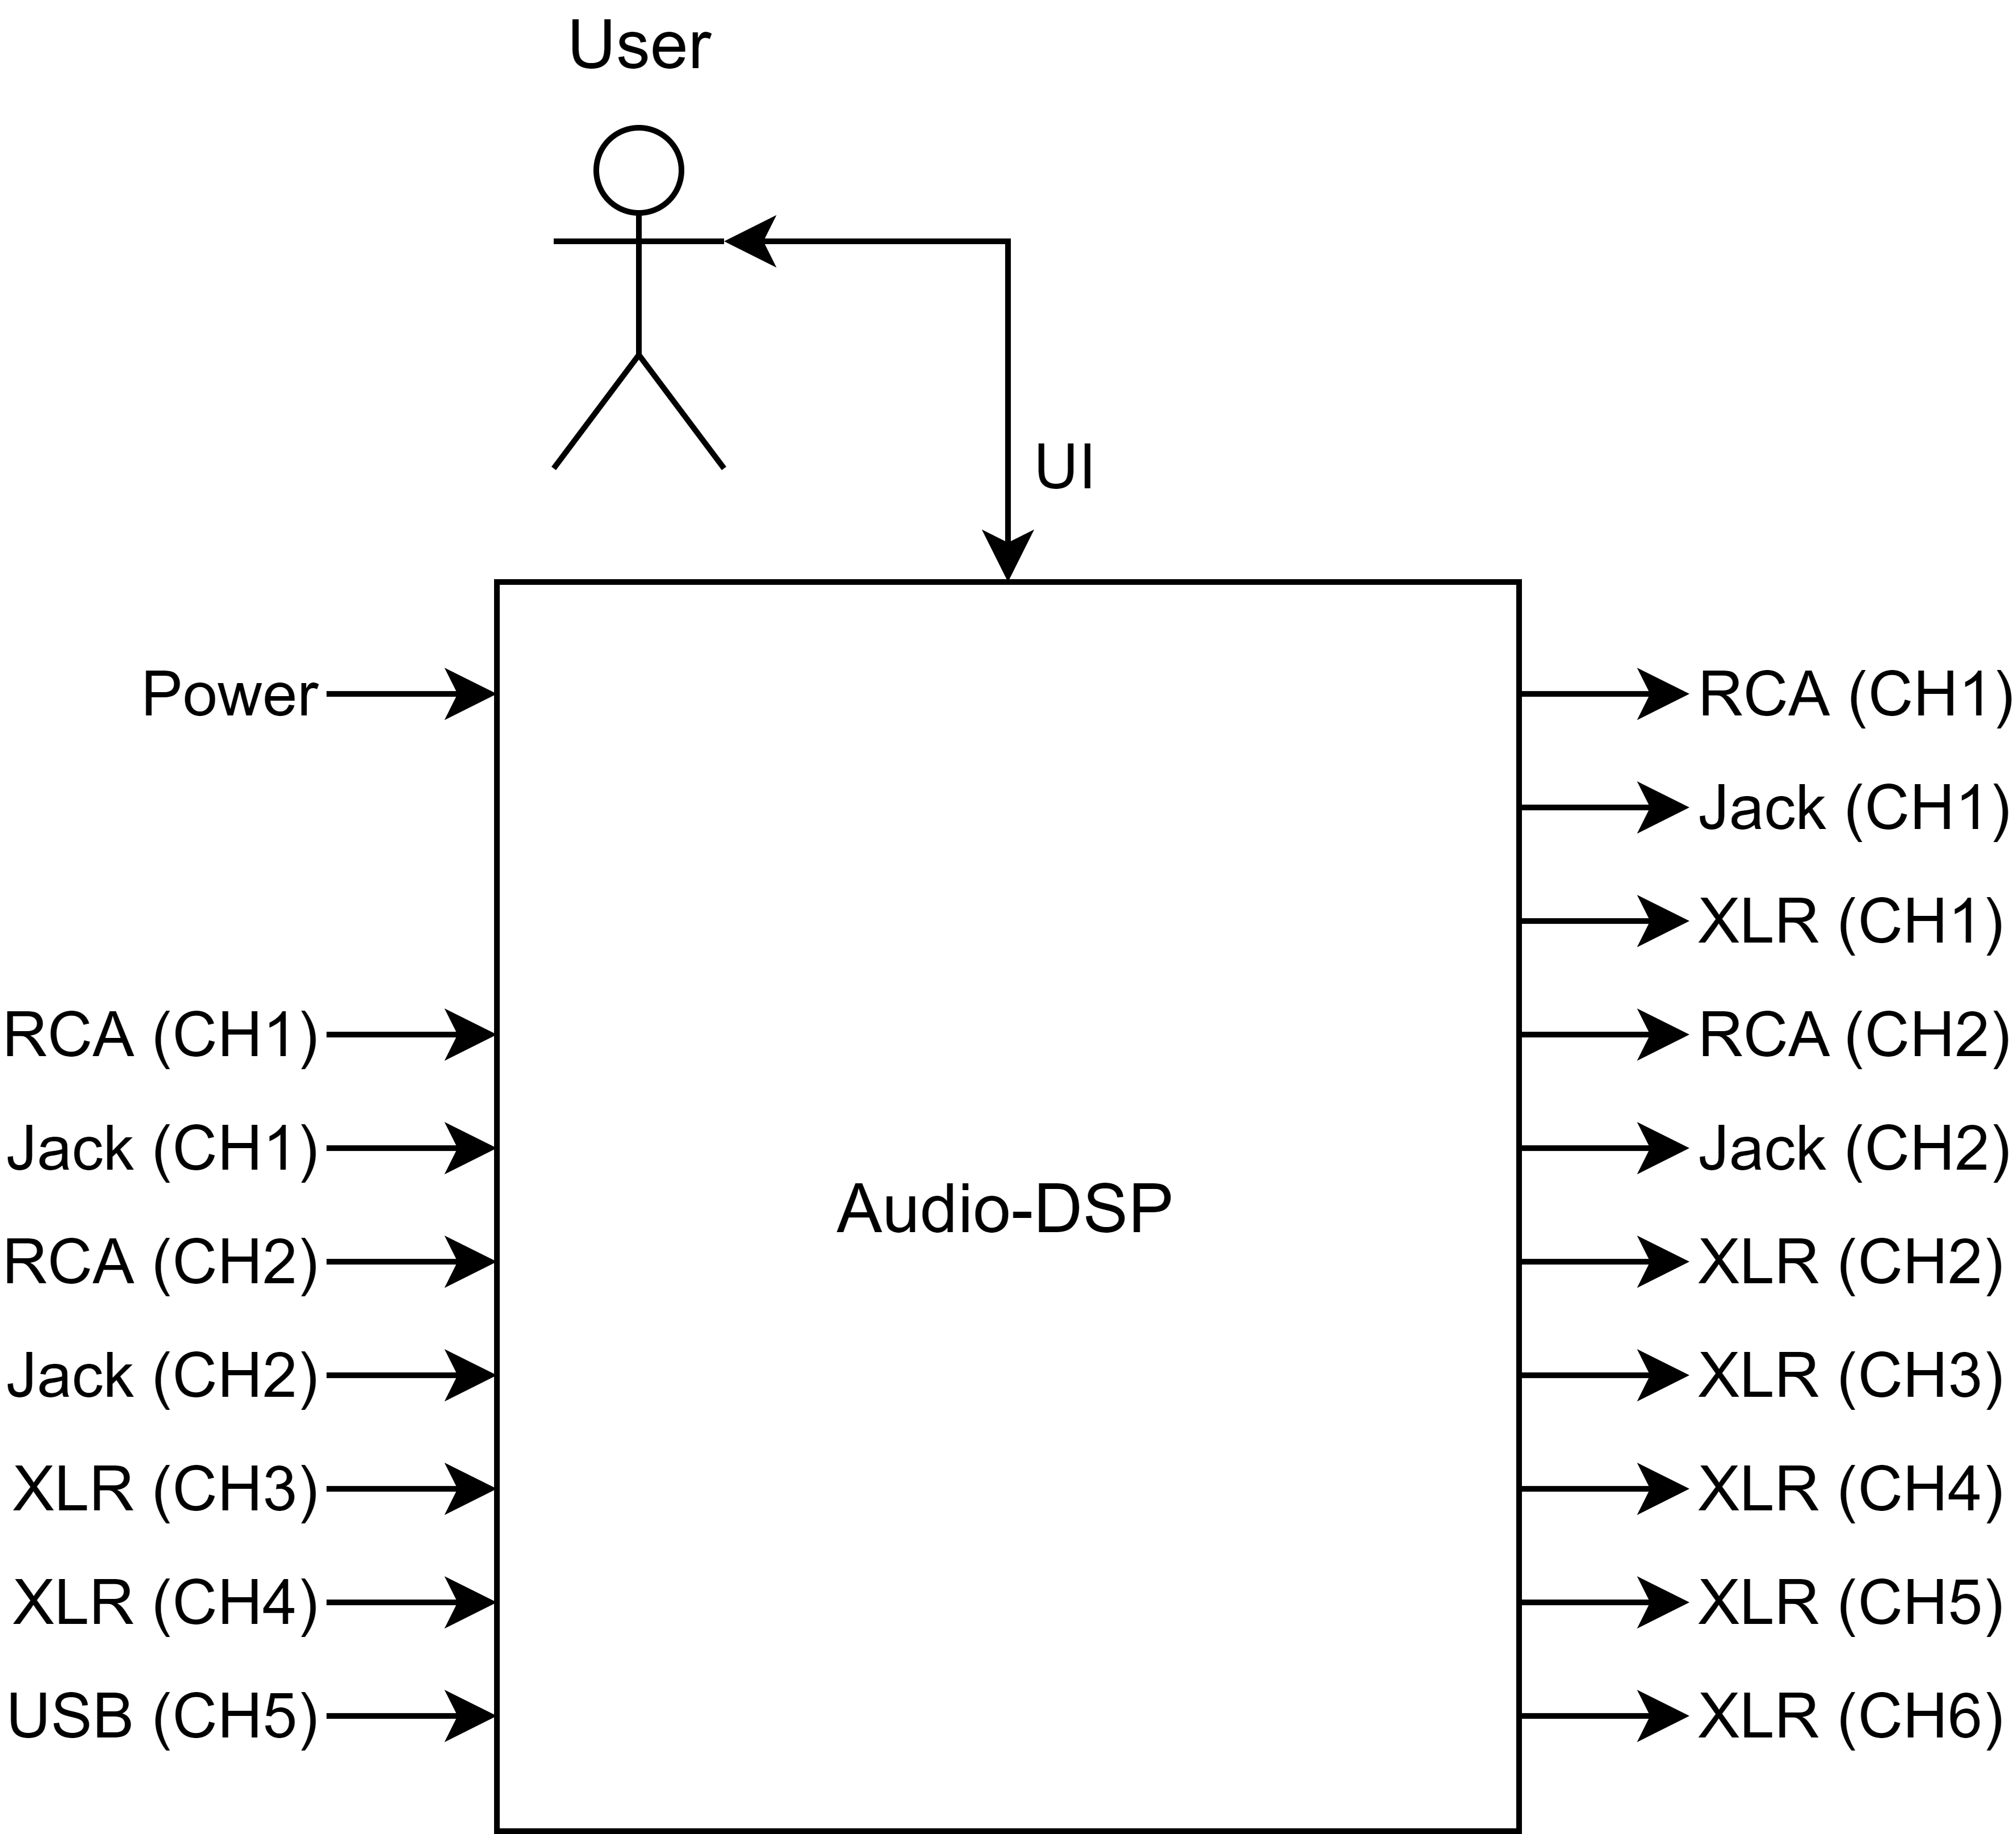
\includegraphics[width=10cm]{Black_box_representation.png}
    \caption{Black box representation}
    \label{fig:Black-box-rep}
\end{figure}